Features  
\begin{itemize}
	\item Qualitative representation - states and transitions
	\item State identification services:
	\begin{itemize}
		\item State details and attribute highlighting - histograms + attribute colors
		\item \lstopar{Timeline + parallel coordinates \cite{parcoords} - when do states occur in time}
		\item \lstopar{Coloring states based on attributes}
		\item Decision trees + rule extraction - Explanation of states
		\item Automatic name generation
		\item Zooming into a state + showing paths from a state
	\end{itemize}
\end{itemize}

When first opening the StreamStory system, the user is presented with a top-level state-transition qualitative representation
of the dataset they have uploaded. System states are represented as circles, while state transitions are
represented by arrows. The size of each state is proportional to the amount of time the system spends in
the state (stationary distribution), while the thickness of an arrow is proportional to the corresponding
transition probability.

The user can use the zoom function to traverse the hierarchy and view the qualitative model on other 
detail levels. When clicking on a state, it becomes selected and several visualization services are
shown, which will be explained in the following subsections.

\subsection{Visual Assistance}

When a state becomes selected, the user interface presents the user with several visual aids which
assist them in identifying the states' meaning. The first of these aids is the timeline histogram
which shows the distribution of the states occurrence over time. An example is shown in Figure 
\ref{fig:time-hist}.

\begin{figure}[h!]
	\centering
	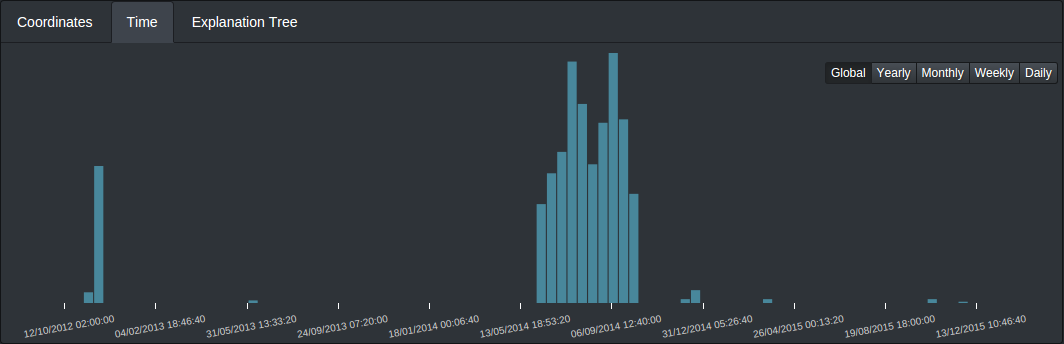
\includegraphics[width=\columnwidth]{timeline}
	\caption{[TODO example decision tree].}
	\label{fig:time-hist}
\end{figure}

[TODO histograms]

\subsection{Automatic Naming}

In order to assist the user in identifying the meaning of states, the system provides automatic default
state names, based on the distribution of attributes in the state. Each state is given a default name
by combining its most outstanding attribute with a discrete level: LOWEST, LOW, HIGH or
HIGHEST.

The attribute and the level are chosen by comparing its distribution inside the state to the global
distribution in all the states through histograms. This is achieved by first computing the percentiles
of the global distribution. The $40^{th}$ percentile is then computed for the state distribution and
compared against the global distribution. If this percentile lies below the $25^{th}$ or $12^{th}$
percentile, the state is marked with LOW or LOWEST respectively. The final name is chosen according
to the attribute which lies in the lowest percentile.


\subsection{Decision Trees and Rule Extraction}

An alternate description of a state is generated through the induction of decision trees. Decision
trees are classification models often used in domains such as medicine for their explanatory power.
When a decision tree is induced, a splitting attribute and cut value are chosen recursively by a
design time criteria. The user can then interpret the tree by traversing the path from the root 
to one of the leafs.

In our use case, we use decision trees as a tool for explaining states. We induce one tree for each
state by classifying the observations form the state against the observations of all other states
thus obtaining a qualitative description of the state. Figure \ref{fig:example-decision-tree} and
Figure \ref{fig:example-decision-tree-rule} show an example decision tree and extracted rules
from a state in the weather dataset presented in section \ref{sec:experiments-weather}.

\begin{figure}[h!]
	\centering
	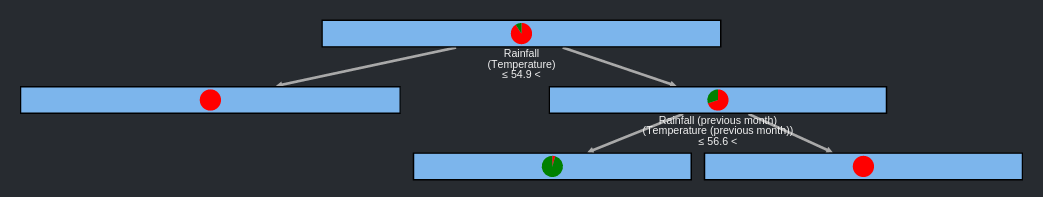
\includegraphics[width=\columnwidth]{tree-rainfall}
	\caption{[TODO example decision tree].}
	\label{fig:example-decision-tree}
\end{figure}

\begin{figure}[h!]
	\centering
	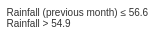
\includegraphics[width=100pt]{rule}
	\caption{[TODO rule generated from decision tree].}
	\label{fig:example-decision-tree-rule}
\end{figure}